\cotefile{81}

\scanpage{43}
que pour \unsure{tt|tout} segment $I$ de $S$, $I\subset S''$, il existe un plus grand segment de $S$ contenu dans $S'$ le contenant.

% slanted
\margin{introduire $\mathrm{Segm}_{\subset S'}(S\deleted{,\unsure{S'}})=\{I\subset S'\mid I\in\mathrm{Segm}(S)\}$}

Les éléments maximaux de $\mathrm{Segm}_{\subset S'}(S\deleted{,\unsure{S'}})$ sont appelés les \uline{segments \unsure{composants|comp.sants}} de la partie $S'$ de $S$.

% slanted
\margin{les élém. maximaux de $\mathrm{Segm}(S,S')$ i.e. les segments composants de $S'$, sont en corr. \unsure{1.1.} \unsure{resp.|pr.} \unsure{avec} les éléments \uline{minimaux} de l'ens des \deleted{\unsure{cl.|cl}} segments de $S$ qui \uline{contiennent} $S''$, par $I\mapsto S\setminus I$
\[
 \mathrm{Seg}_{\subset S'}(S)\overset{\unsure{\mathrm{antiiso.}}}{\simeq}\mathrm{Seg}_{\supset S''}(S)
\]}

Ils forment une partition de $S'$, d'où une relation d'équivalence dans $S'$.

En termes d'une réalisation top. de $(S,\{u,u^{-1}\})$ par un polygone top $(X,S)$, si $S''=S\setminus S'$, les \deleted{classes} segments de $S'$ sont en corr biunivoque avec les comp. conn. de $X\setminus S''$ qui rencontrent $S'$ -- ce sont les intersections de $S'$ avec ces comp. connexes.
\figure{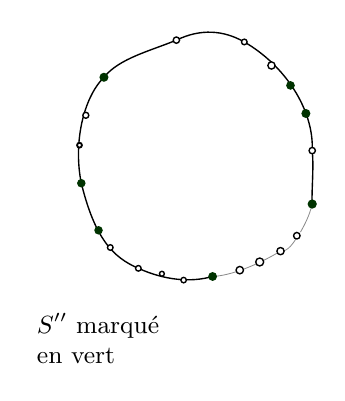
\begin{tikzpicture}[x=1.15cm,y=1.15cm,line width=.5pt]
\draw (-1.01,.97) .. controls (-.84,1.18) and (-.50,1.26) .. (-.21,1.38)
 .. controls (.06,1.51) and (.31,1.49) .. (.54,1.36)
 .. controls (.99,1.10) and (1.31,.61) .. (1.29,.16)
 .. controls (1.31,-.03) and (1.28,-.31) .. (1.29,-.43);
\draw[black!45,line width=.3pt] (1.29,-.43) .. controls (1.26,-.56) and (1.20,-.67) .. (1.16,-.74);
\draw[black!45,line width=.3pt] (1.13,-.78) .. controls (1.06,-.91) and (.99,-.96) .. (.94,-.95)
 .. controls (.69,-1.10) and (.40,-1.22) .. (.19,-1.23);
\draw (.19,-1.23) .. controls (-.06,-1.30) and (-.34,-1.27) .. (-.63,-1.14)
 .. controls (-.91,-1.02) and (-1.11,-.81) .. (-1.26,-.20)
 .. controls (-1.35,.24) and (-1.24,.74) .. (-1.01,.97);
\foreach \x/\y/\r in {-.21/1.38/.035,.54/1.36/.031,.84/1.10/.04,1.29/.16/.035,1.12/-.78/.036,.94/-.95/.04,.71/-1.07/.044,.49/-1.16/.041,-.13/-1.27/.03,-.37/-1.20/.027,-.63/-1.14/.031,-.94/-.91/.031,-1.21/.55/.033}
  \draw[fill=white] (\x,\y) circle[radius=\r];
\draw[line width=.65pt,fill=white] (-1.28,.22) circle[radius=.027];
\foreach \x/\y/\r in {-1.01/.97/.05,1.05/.88/.048,1.22/.57/.05,1.29/-.43/.051,.19/-1.23/.049,-1.07/-.72/.047,-1.26/-.20/.047}
  \fill[green!20!black] (\x,\y) circle[radius=\r];
\node[anchor=north west,align=left,font=\small] at (-1.86,-1.53) {$S''$ marqué\\en vert};
\end{tikzpicture}}

\uline{Proposition} Soient $A,B$ deux parties \deleted{disjointes non vides} de $S$, on suppose \deleted{$A$ et $B$}
\[
 A,B\ne\phi,S,\qquad A\cap B=\phi.
\]

Conditions équivalentes

% slanted
\margin{\uline{NB} On peut \inserted{prendre} pour $\bar A,\bar B$ les \inserted{\unsure{plus|des}} \deleted{\unsure{petits}} \deleted{\unsure{segments|sgmts}} composants}

a) $\exists$ segments $\bar A,\bar B$ de $S$, tels que $\bar A\supset A,\bar B\supset B$, $\bar A\cap\bar B=\phi$
% archive sheet number: 42

\scanpage{44}
b) Pour $a,\deleted{\unsure{b'}}a'\in A$, $b,b'\in B$, avec $a\ne a'$, $b\ne b'$, \deleted{\unsure{les ordres|les ord.}} $a,a'$ sont \deleted{\uline{contigus}} \inserted{adjacents} pour la structure bi-circularisée sur \inserted{l'ens à 4 éléments} $\{a,a',b,b'\}$ induite par celle de $S$, \deleted{i.e. ils}. ($\Longleftrightarrow\{b,b'\}$ sont \deleted{contigus} \inserted{adjacents} $\Longleftrightarrow\{a,a'\}$ ne sont pas opposés $\Longleftrightarrow b,b'$ ne sont \unsure{opposés|voisins}

c) $B$ est contenu dans un segment composant de $S\setminus A$

c$'$) $A$ est contenu dans un segment composant de $S\setminus B$

% slanted
\margin{d) Quand $S$ est réalisé comme \inserted{une partie} d'un disque \inserted{convexe} plongé dans un plan réel affine)\,: Soit $P_A$ la réunion des segments affines joignant deux à deux les points de $A$ (ou, \unsure{au choix|au besoin}, l'enveloppe convexe de $A$) alors $P_A\cap P_B=\phi$}

Quand il en est ainsi, \unsure{Parmi|parmi} les couples $(\bar A,\bar B)$ \inserted{de segments} satisfaisant les conditions de a), il existe un plus petit\ldots

On dit que $A,B$ sont \uline{non panachés}

(\uline{Ex} si \deleted{\unsure{$A$ et}} $A$ ou $B$ réduit à un pt. \inserted{(plus général\textsuperscript{t} si $A$ ou $B$ est un segment}

Si $A$ et $B$ sont de cardinal 2, cel. signifie que, sur $A\cup B$ pour la bicircularisation induite, $A$ est un côté du carré $A\cup B$ (i.e. encore que $B$ est un côté). Dans le cas général, $A$ et $B$ sont non panachés ssi $\forall\, A'\in\unsure{\mathfrak P_2|\mathcal P_2|P_2}(A)$, $B'\in\mathfrak P_2(B)$, $A'$ et $B'$ sont non panachés.

% slanted
\margin{\deleted{e) \unsure{On a} $A,B\subset C$, \unsure{$C=$|un} segment \unsure{on a des} $\bar A,\bar B$ \unsure{ds|de} \unsure{st} $\bar A\cap\bar B=\phi$, \unsure{$=\ A$}}}

% slanted
\margin{\uline{Cor} De plus, \unsure{lorsque ces} conditions \unsure{sont} sauf dans le cas où $A\sqcup B=S$ (\unsure{donc|alors} $A$ et $B$ des segments compl. l'un de l'autre), quand il existe \inserted{\uline{\unsure{donc|deux}}} un segment $C\supset A\cup B$, on peut prendre pour $\bar A,\bar B$ ds a) les \unsure{composants de $A$ et $B$|composantes de $A$ et $B$} $\subset C$.}
% archive sheet number: 43

\scanpage{45}
\uline{Structure à étudier} Partition de $S$ en des $(S_\alpha)_{\alpha\in J}$ mutuellement non panachées. (On les appelle des partitions non \unsure{panachées|panachés})

% slanted
\margin{\uline{Ex} partition grossière, \unsure{ayant} juste une classe, égale à $S$\unsure{.\,--|\ldots}}

\uline{Intuition} À \deleted{\unsure{une tel|un tel}} un ens. bicircularisé avec partition non panachée, \inserted{de \deleted{\unsure{Card.}} \unsure{Cardinal|cardinal} $N$,} correspond (fonctoriellement pour les iso) un ens. bicircularisé (de \deleted{\unsure{cardin|cardinal}} \unsure{Cardinal|cardinal} \inserted{\uline{pair}} $N'\leq N$), avec une partition \inserted{non panachée} de degré 2 (classes de cardinal 2).\,-\,---

\figure{\begin{tikzpicture}[x=.01cm,y=-.01cm,line cap=round,line join=round]
\draw[line width=.68pt] (578,1785)
 .. controls (603,1770) and (623,1748) .. (638,1710);
\draw[line width=.42pt] (638,1710)
 .. controls (661,1653) and (677,1603) .. (686,1546)
 .. controls (694,1496) and (685,1453) .. (666,1410);
\draw[line width=.68pt] (666,1410)
 .. controls (631,1336) and (535,1277) .. (446,1281)
 .. controls (350,1282) and (267,1322) .. (211,1385)
 .. controls (174,1424) and (158,1480) .. (156,1542);
\draw[line width=.45pt] (156,1542)
 .. controls (152,1563) and (153,1586) .. (157,1608);
\draw[line width=.68pt] (157,1608)
 .. controls (164,1687) and (211,1733) .. (282,1794)
 .. controls (325,1830) and (374,1861) .. (425,1857)
 .. controls (507,1855) and (569,1831) .. (601,1781);
\end{tikzpicture}}
% archive sheet number: 44

\scanpage{46}
Soit $\Sigma$ un ens. de segments de $S$, satisfaisant la condition suivante

($\deleted{\unsure{\Sigma|>}}\sigma$ 1) Si $A,B\in\Sigma$, et si $A\cap B\ne\phi$, alors $A\subset B$ ou $B\subset A$. \inserted{($\sigma.2$)} Si de plus $A\ne B$ et $A\subset B$, alors $A$ ne contient pas d'extrémité de $B$.

Posons alors, pour $A\in\Sigma$
\[
 A^*=\unsure{.|\cdot}\, A\setminus\bigcup_{\substack{B\in\Sigma\\ B\subset A\\ B\ne A}} B
\]
On a (par $\sigma.2$)
\[
 A^*\supset\partial A\quad\text{(ens des extrémités de $A$)}
\]
donc $A^*\ne\phi$. Je dis que
\[
 \begin{aligned}
 A&\longmapsto A^*\\
 \Sigma&\longrightarrow \unsure{P|\mathcal P|\mathfrak P}(S)
 \end{aligned}
 \qquad\text{est injectif}
\]
% slanted
\margin{\uline{Prop} Si $A,B\in\Sigma$, $A\ne B$, alors $A^*\cap B^*=\phi$ (donc $A^*\ne B^*$). \deleted{\unsure{sont disj.|sont di}} et $A^*,B^*$ non panachés. On a $\bigcup_{A\in\Sigma} A=\bigcup_{A\in\Sigma} A^*$. Si $x\in\bigcup_{A\in\Sigma}A$, alors l'ens \inserted{$\Sigma(x)$} des $A\in\Sigma$ tels que $x\in\Sigma$ est tot. ordonné, donc admet un plus petit \unsure{élément|élém\textsuperscript{t}}, soit $A$, et alors $A^*\ni x$.}
i.e. que si $A,B\in\Sigma$, alors
\[
 A^*=B^*\quad\Longrightarrow\quad A=B
\]
\inserted{i.e. $A\ne B$ \deleted{distincts} $\Longrightarrow A^*\ne B^*$. Comme $A^*,B^*$ sont $\ne\phi$, il suffit de prouver $A^*\cap B^*=\phi$.} \deleted{En effet}, si $A\cap B=\phi$, alors $A^*\cap B^*=\phi$, donc $A^*\ne B^*$ (puisque $A^*,B^*$ non vides). Si $A\cap B\ne\phi$, \unsure{on a|$\cdots$} \inserted{(par $\sigma\,1$)} $A\subset B$ ou $B\subset A$, soit $A\subset B$.

\deleted{Mais alors $A\cap\partial B=\phi$ \inserted{par $\sigma 2$}, \deleted{donc} $A^*\cap\partial B=\phi$, donc \unsure{$A^*\supset$|$A\supset$} (comme $\phi\ne\partial B\subset B^*$) $A^*\not\supset B^*$. Comme \unsure{on aurait|on a} $A^*\cap\partial B=$} Comme $A\ne B$, $A\cap B^*=\phi$ par définition de $B^*$, donc $A^*\cap B^*=\phi$, \unsure{qfd.|cqfd.} \deleted{Je dis} Aussi, $A^*,B^*$ non panachés, puisque $A^*\subset A$ segment $\subset S\setminus B^*$.
% archive sheet number: 45

\scanpage{47}
\uline{\unsure{Conséquence|Conséquences}}: Si $\bigcup_{A\in\Sigma}A^*=S$, alors \deleted{les} $(A^*)_{A\in\Sigma}$ est une partition \deleted{\unsure{des|sans|dans}} \unsure{non} panachée de $S$. Si $\bigcup_{A\in\Sigma}A^*\ne S$, alors posant
\[
 \deleted{\unsure{R,\Sigma|R\ \Sigma}}\mathpunct{.}\qquad
 \left\{\begin{aligned}
 R&=S\setminus\bigcup_{A\in\Sigma}A^*,\\
 R^*&=R\setminus\bigcup_{\substack{A\in\widehat\Sigma\\ A\subsetneq R}}A=R
 \end{aligned}\right.\qquad
 \begin{aligned}
 \widehat\Sigma&=\Sigma\cup\{R\}\\
 &\deleted{\unsure{\Sigma|\in\Sigma|\ne\Sigma_0}}
 \end{aligned}
\]
alors $(A^*)_{A\in\widehat\Sigma}$ est une partition non panachée de $S$.

\uline{NB} Si $R$ est lui-= un segment, alors \deleted{\unsure{l'intérêt} \unsure{de le prendre|de le joindre}} $\widehat\Sigma$ satisfait les conditions de $\Sigma$ -- et $R$ est un élément \deleted{``\unsure{sp.|spéc.}} ``isolé'' de $\widehat\Sigma$, en ce sens que \inserted{pour} \unsure{tt|$A$|$\forall$} autre \unsure{élément|élém} \inserted{$A$} de $\widehat\Sigma$, \deleted{\unsure{on}}. $R\cap A=\phi$ -- \deleted{\unsure{donc}} \inserted{i.e.} $R$ est \unsure{:|à} la fois minimal, et maximal. Considérons
\[
 \begin{aligned}
 (\sigma\ 3)\qquad R=S\setminus\bigcup_{A\in\Sigma}A\;
 \bigl(=S\setminus\bigcup A^*\bigr)&\quad\text{n'est}\\
 &\quad\text{pas un segment}
 \end{aligned}
\]
(NB \deleted{\unsure{p.ex|p.}}\inserted{\unsure{c'est}} le cas si $R=\phi$ p. ex)

% slanted
\margin{faux}
Montrons dans ce cas que \deleted{\unsure{on a|est}} $\Sigma$ est \deleted{défini} \inserted{\unsure{connu|connus}} quand on connait la partition $\widehat\Sigma^*=\{A^*\mid A\in\widehat\Sigma\}$

\[
 \bigl(\text{où }\widehat\Sigma=\left\{\begin{aligned}
 &\Sigma\quad\text{si }R=\phi\\
 &\Sigma\cup\{R\}\quad\text{si }R\ne\phi
 \end{aligned}\right.\bigr)
\]
% archive sheet number: 46

\scanpage{48}
Je veux caractériser $A$ en termes de $\widehat\Sigma^*, A^*\in\widehat\Sigma^*$ (dans le cas $A\in\Sigma$). Bien sûr, $A$ est un \deleted{\unsure{segt|segt.}} segment qui contient $A^*$, et comme $A^*\supset\partial A$, il est minimal (\deleted{\unsure{l'unique|l'un}} qui convient) parmi les segments \inserted{de $S$} qui conti\deleted{\unsure{ent}}ennent $A^*$ -- mais cela ne suffit pas à le caractériser. Il a cependant la propriété supplémentaire,
\[
 \forall B^*\in\widehat\Sigma^*,\quad\text{\unsure{on a}}\quad B^*\cap A=\phi,\quad\text{ou }B^*\subset A
\]

\uline{NB} En fait, avec les seules conditions $\sigma1:\sigma3$ sur $\Sigma$, \deleted{\unsure{c'|en|i}} il n'est pas vrai que la connaissance de $\widehat\Sigma^*$ redonne $\Sigma$, exemple

\figure{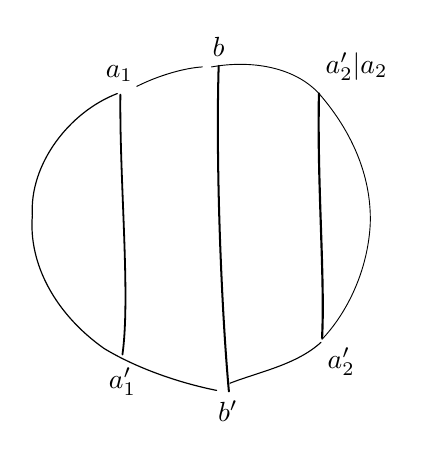
\begin{tikzpicture}[x=.013cm,y=-.013cm,line cap=round,line join=round]
\draw[line width=.43pt] (232,1287) .. controls (185,1305) and (146,1356) .. (149,1406) .. controls (145,1453) and (171,1502) .. (219,1536) .. controls (252,1556) and (294,1570) .. (329,1577);
\draw[line width=.35pt] (251,1280) .. controls (273,1269) and (298,1262) .. (315,1261);
\draw[line width=.33pt] (324,1261) .. controls (363,1254) and (405,1261) .. (429,1287) .. controls (463,1326) and (481,1371) .. (479,1416) .. controls (476,1464) and (454,1504) .. (432,1527);
\draw[line width=.40pt] (431,1530) .. controls (407,1552) and (370,1559) .. (342,1570);
\draw[line width=.65pt] (235,1288) .. controls (234,1372) and (245,1485) .. (237,1542);
\draw[line width=.73pt] (331,1260) .. controls (328,1360) and (334,1502) .. (341,1578);
\draw[line width=.78pt] (429,1287) .. controls (427,1374) and (435,1468) .. (432,1526);
\node[above] at (234,1285) {$a_1$};
\node[above] at (331,1260) {$b$};
\node[above right] at (426,1284) {$\unsure{a'_2|a_2}$};
\node[below] at (237,1545) {$a'_1$};
\node[below] at (340,1578) {$b'$};
\node[below right] at (428,1526) {$a'_2$};
\end{tikzpicture}}
relation d'équiv. \inserted{$\mathcal R$} avec trois classes $\{a_1,a'_1\}$ $\{b,b'\}$ $\{a_2,a'_2\}$, \inserted{\unsure{définir ici|définissons}} $\Sigma_1$ formé des segments $\{a_i,a'_i\}$ \deleted{$\{a,a'\}$} $(i\in\{1,2\})$, et $\{a_1,a'_1,b,b'\}$ et $\Sigma_2$ défini de façon symétrique, définissent la $=$ $\mathcal R$\unsure{.|*}

\deleted{\unsure{Exemple|Énoncé} plus général: on \unsure{peut} de façon \unsure{unique} \unsure{donner} $\Sigma$ de façon à donner}
\[
 \begin{aligned}
 &\left\{\begin{aligned}
   &\deleted{\widehat\Sigma^*=\mathcal R,\quad\text{\uuline{et}}}\\
   &\deleted{\dot R\overset{\text{déf}}{=}S\setminus\coprod_{A\in\Sigma} A=\unsure{S'|S_1|S_i},}
 \end{aligned}\right.\\
 &\qquad\deleted{\text{\unsure{élém\textsuperscript{t}|élément} \uline{donné} d'}}\\
 &\qquad\deleted{\text{avance de }\mathcal R}\\
 &\qquad S'\ \text{non un segment}
 \end{aligned}
\]
% archive sheet number: 47

\scanpage{49}
$\unsure{R|\mathcal{R}}$ relation d'\unsure{équiva|équiv.} non \unsure{panachée|ponctuelle} sur $S$.

\uline{Segments} \inserted{$\underline{\mathcal{R}}$} \uline{saturés} : \unsure{stable|st.bl|stables} par passage au \unsure{complémentaire|complémentation}, et par intersection et réunion quand celles-ci \deleted{\unsure{d}}donnent des segments (\inserted{p. ex. si} $A\cup B\ne S$, $A\cap B\ne\phi$)

Si $S_i\in\mathcal{R}$, alors les segments composants de $\complement S_i$ sont saturés, donc aussi leurs complémentaires i.e. les segments minimaux contenant $S_i$ (ou \inserted{segments} cocomposants de $S_i$). \deleted{Plus \unsure{général\textsuperscript{mt}|généralement}, \unsure{Si|si} $T\subset S$ est une partie de $S$ $R$-saturée, alors les segments composants de}

\noindent\llap{\rule[-.92\baselineskip]{.4pt}{1.8\baselineskip}\hspace{.35em}}\uline{Prop} Les segments saturés minimaux sont les $\deleted{\unsure{A|S}}S_i\in R$ qui sont des segments.

% slanted
\reversemarginpar\margin{On appelle les parties des \uline{\unsure{onglets|anglets}}}

Il est évident que si $S_i\in\deleted{\unsure{A}}R$ est un segment, alors c'est un segment saturé, et il est minimal parmi ces derniers (et $=$ parmi les parties saturées non vides). Inversement, soit $A$ segment saturé minimal, \deleted{\unsure{soit}} soit $S_i\in R$, $S_i\subset A$, \deleted{soit} \unsure{je|Je} dis que $S_i=A$, \deleted{\unsure{ou|sin}} i.e. que l'on ne peut avoir $S_i,S_j\in R$ distincts, et
% slanted
\margin{\unsure{oubli|oublié} du côté de la \unsure{question|section|notion|notation}}
\par\noindent\begin{minipage}[t]{.23\linewidth}
\vspace{0pt}
\figure{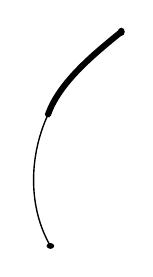
\begin{tikzpicture}[x=1cm,y=1cm,line cap=round,line join=round]
  \draw[line width=.5pt] (.18,0) .. controls (-.10,.48) and (-.10,1.13) .. (.15,1.67)
    .. controls (.30,2.10) and (.79,2.48) .. (1.08,2.72);
  \draw[line width=2.2pt] (.15,1.67) .. controls (.30,2.10) and (.79,2.48) .. (1.08,2.72);
  \fill (.18,0) ellipse [x radius=.049,y radius=.037];
  \fill (1.08,2.72) ellipse [x radius=.044,y radius=.052];
\end{tikzpicture}}
\end{minipage}\hfill\begin{minipage}[t]{.73\linewidth}
\vspace{0pt}
$\subset A$. En effet, si $A_i$ $(A_j)$ est le segm cocomposant de $\deleted{\unsure{A}}S_i$ qui est contenu dans $A$, alors la condition que $S_i,S_j$ sont \deleted{\unsure{dis}}\unsure{non|bien} panachés s'exprime par la condition que $A_i\cap A_j=\phi$, donc $A_i,A_j$ sont des segments saturés $\subset A$ et $\ne A$, absurde.
\end{minipage}
\normalmarginpar
% archive sheet number: 48

\scanpage{50}
\uline{Cor} Tout \deleted{\unsure{conti|cont}} segment saturé contient un onglet -- donc si $\mathcal{R}$ n'est pas la relation grossière il existe au moins deux onglets (car il existe alors au moins deux segments saturés, complémentaires l'un de l'autre)

Soit \inserted{$\unsure{\Sigma_{1}|\Sigma_{0}}$ l'ens des onglets de $R$,} $\deleted{\unsure{S_{0}|S_1}}\unsure{T_{1}|T_{0}}$ la réunion des onglets, $\deleted{\unsure{S_1}}R_1$ son complémentaire. Alors, si $\deleted{S_1}R_1\ne\phi$, $\deleted{S_1}R_1$ a au moins deux segments composants ($\operatorname{card}\unsure{\pi_0|\Pi_0}(R_1)\geq 2$), sinon $R_1$ serait un \deleted{\unsure{s}}segment donc contiendrait un onglet, absurde. Si $\operatorname{card} R_1=2$, alors $R_1\in\mathcal{R}$ \deleted{est un} donc $\mathcal{R}$ consiste en les onglets et en $R_1$, (car \deleted{\unsure{$R_1$|$R$}} les $\unsure{S_i|S'}\subset R_1$ sont de card. $\geq 2$, \deleted{\unsure{puis|puisq}} car ceux de cardinal $1$ seraient des onglets \ldots)

Si $\operatorname{card} R_1\geq 3$, $R_1$ est lui $=$ un graphe polygonal; et $\mathcal{R}_1=\mathcal{R}\vert R_1$ est une relation d'équivalence non panachée. De plus, \deleted{\unsure{al|Au}}Aucun $\unsure{S_i|S_1}\in\mathcal{R}_1$ n'est contenu dans un segment composant de $R_1$ -- sinon il serait contenu dans un segment saturé contenu dans $\deleted{\unsure{S_1}}R_1$ (\unsure{Savoir|savoir} son cocomposant contenu dans ce composant), lequel contiendrait un onglet $\subset R_1$ -- absurde. Si $\mathcal{R}_1$ est la relation grossière, on a fini -- $\mathcal{R}$ est formée des onglets, et de $R_1$.
% margin note written sideways
\margin{\unsure{Construction|Conclusion} \unsure{fausse}}
% archive sheet number: 49

\scanpage{51}
Sinon, considérons l'ens des \inserted{$\mathcal{R}_1$-}\unsure{onglets|anglets}, \deleted{\unsure{dis|des|de}} -- il y en a au moins deux. \inserted{Aussi l'un de} ces onglets est en corr. $1$-$1$. avec un ens. de \unsure{(}segments $\Sigma_2$ de $S$, dont chacun contient un composant au moins de $\deleted{S_1}T_1$, et dont les extrémités sont (\deleted{\unsure{di|dis}}distinctes et) dans $S_1$, et qui \unsure{sont} mutuellement disjoints. Soit $T_2$

\diagram{$\begin{array}{ccccc}\Sigma_1&\Sigma_2&\Sigma_3&-&\Sigma_i\\[3pt]T_1&T_2&T_3&&T_i\end{array}$}

$\Sigma_i$ est un ens. de segments \inserted{($R$-\unsure{saturés|admis})} mutuellement disjoints, $\operatorname{card}\Sigma_i\geq 2$, \unsure{$\cdot$|.} de réunion $T_i'$ \inserted{(\uline{NB} les \unsure{segm.|segmts|segm} composants de $T_i$ sont donc des réunions partielles de $\Sigma_i$, donc saturés)}

\reversemarginpar\margin{\deleted{$i\unsure{\geq|\to}$}}
\[\inserted{T_i=T_i'\cup T_{\unsure{i-1|i}}}\]
\margin{$i\geq 2$ \deleted{\unsure{donc}}}
\noindent\llap{\rule[-2\baselineskip]{.4pt}{3\baselineskip}\hspace{.4em}}\deleted{Tout élément $A\in\Sigma_{i-1}$ est contenu dans un $\deleted{\unsure{A}}B\in\Sigma_i$, \unsure{les|tout|tel}}

Tout $B\in\Sigma_i$ contient au moins un \deleted{$A\in\Sigma_{i-1}$}\inserted{\uline{segment composant}} \deleted{\unsure{de}} de $T_{i-1}$, et $\partial B\subset S\setminus T_{i-1}$ \deleted{$\unsure{\partial B|B}$}\normalmarginpar

\noindent\begin{minipage}[t]{.46\linewidth}
$\Sigma_1$ ens de segments \unsure{mut\textsuperscript{t}|mut\textsuperscript{lt}} disj. de $S=S_0$, \deleted{\unsure{de cardinal}} \inserted{$\operatorname{card}(\Sigma_1)\geq 2$}
\[T_1=\bigcup_{A\in\Sigma_1} A,\quad S_1=S\setminus T_1\]
\[\deleted{\operatorname{card}S_1\geq\unsure{3|2}}\]
les segm. comp. de $S_1$ dans $S$ au nb au moins $2$
\end{minipage}\hfill\begin{minipage}[t]{.51\linewidth}
$\Sigma'_2$ ens de segm. mut. disjoints \uline{de $S_2$} \uline{non} \uline{contenus} dans un des segments composants
\[\begin{aligned}\operatorname{card}\Sigma_1&\geq 2,\\
T_2&=T_1\cup\mathop{\deleted{\Sigma}\bigcup}\limits_{A\in\Sigma'_2} A\\
\deleted{\unsure{C|\Sigma|S}}S_2&=S\setminus T_2\\
\operatorname{card}\unsure{\pi_0|\Pi_0}(S_2)&\ne 1
\end{aligned}\]
\end{minipage}
% archive sheet number: 50

\scanpage{52}
$I$ graphe-segment (fini) ayant au moins deux sommets

Deux parties d'éléments $\varepsilon,\varepsilon'\in\unsure{\mathcal{P}_2|\mathfrak{P}_2|P_2}(I)$ sont dites \uline{non panachées} si \inserted{$\varepsilon\cap\varepsilon'=\phi$ et si} $I_{\varepsilon}\cap I_{\varepsilon'}=\phi$ \inserted{ou $I_{\varepsilon}\subset I_{\varepsilon'}$ \uline{ou} $I_{\varepsilon'}\subset I_{\varepsilon}$}, -- $I_{\varepsilon}$ est le segment déterminé par un ens. à deux éléments $\varepsilon$.

Deux parties $A,A'$ de $I$ sont dites non panachées si
\[
\begin{aligned}
\text{a)}\quad &A\cap A'=\phi\\
\text{b)}\quad &\forall\,\varepsilon\in\mathcal{P}_2(A),\quad \varepsilon'\in\mathcal{P}_2(A'),\quad \varepsilon,\varepsilon'\ \text{non panachés}
\end{aligned}
\]

% slanted
\reversemarginpar\margin{ou encore, que l'un des deux $A,B$ est contenu dans un segment qui ne rencontre \unsure{pas} l'autre}
Cela revient au $=$ de dire que $A'$ est contenu dans l'un des \deleted{\unsure{intervalles}}\inserted{segments} composants de $I\setminus A$ \uline{ou} (si $A$ ne contient pas d'extrémités de $I$) dans la réunion des deux compos. \deleted{\unsure{de|des}} \unsure{extrêmes|extremes} (i.e. ceux qui contiennent les deux extrémités

% slanted
\margin{\uline{NB} un segment peut être réduit à un seul sommet --}\normalmarginpar

Partitions non panachées de $I$

Ens \inserted{$\Sigma$} de segments de $I$ qui est :

a) Si $A\unsure{,}B\in\Sigma$, on a $A\cap B=\phi$, ou $A\subset B$ ou $B\subset A$

b) Si $A,B\in\Sigma$, $\deleted{\unsure{A|B}}B\subsetneq A$, alors $B\deleted{\unsure{=|A}}\unsure{\cap}\partial A=\phi$

c) \deleted{\unsure{$\forall$|$\forall\varepsilon$}}\unsure{On a|on a} $\partial I\subset\bigcup\limits_{A\in\Sigma} A$ donc $\partial I\subset\bigcup\limits_{A\in\Sigma}\partial A$

Pour un tel $\Sigma$, posons pour $A\in\Sigma$
\[
A^{\ast}=A\setminus\bigcup_{\substack{B\in\Sigma\\B\subset A}} B \qquad (\supset\partial A)
\]
\margin{donc $A^{\ast}\ne\phi$}

alors \deleted{les $A^{\ast}$, \unsure{s\textsuperscript{t}|à|$A$} deux à de} pour $A,B\in\Sigma$, $A\ne B$, on a $A^{\ast}$ et $B^{\ast}$ non panachés -- posons \deleted{\unsure{$\Sigma$|$\hat{\Sigma}$|en}} \unsure{alors|les|l'ens} \deleted{$R=$}
\[
I'=\bigcup_{A\in\Sigma}A=\bigcup_{A\in\Sigma} A^{\ast},\quad R=I\setminus I',\quad R^{\ast}=R
\]
\[
\hat{\Sigma}=\begin{cases}
\Sigma &\text{si }R=\phi\\
\Sigma\cup\{R\} &\text{si }R\ne\phi
\end{cases}
\]
% archive sheet number: 51

\scanpage{53}
alors \[ \hat{\Sigma}^{\ast}=\{A^{\ast}\mid A\in\hat{\Sigma}\} \] est une partition non panachée de $I$.

\uline{NB} Toute partition non panachée peut s'obtenir ainsi, mais de plusieurs façons \ldots\,-

Soit $\Sigma_{\unsure{\mathrm{max}|\mathrm{ma}}}$ l'ens des éléments maximaux de $\Sigma$. On voit de suite que deux \unsure{élémts|éléments} distincts de $\Sigma_{\mathrm{max}}$ sont disjoints, et que \[ I'=\bigcup_{A\in\Sigma_{\mathrm{max}}}A \]
% archive sheet number: 52

\scanpage{54}
\noindent\begin{minipage}[t]{.47\linewidth}
\figure{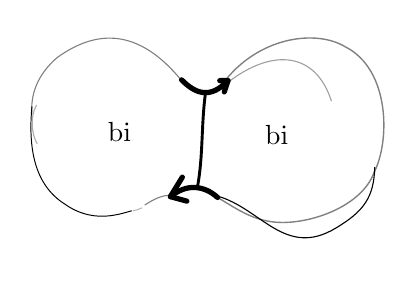
\begin{tikzpicture}[x=.0095cm,y=-.0095cm,line cap=round,line join=round]
  \draw[gray,line width=.4pt] (278,145) .. controls (221,75) and (165,76) .. (112,114) .. controls (85,137) and (76,164) .. (78,190);
  \draw[line width=.35pt] (78,180) .. controls (73,235) and (81,284) .. (122,310) .. controls (159,336) and (193,324) .. (211,319);
  \draw[gray!60,line width=.35pt] (213,319) .. controls (217,319) and (221,316) .. (225,315);
  \draw[gray,line width=.4pt] (229,311) .. controls (242,303) and (251,298) .. (265,298);
  \draw[gray!65] (84,178) .. controls (75,194) and (78,218) .. (85,229);
  \draw[gray,line width=.5pt] (333,149) .. controls (380,86) and (458,76) .. (497,100) .. controls (556,130) and (557,225) .. (535,268) .. controls (517,317) and (438,341) .. (395,333) .. controls (365,328) and (344,311) .. (319,297);
  \draw[gray!75] (339,148) .. controls (402,99) and (458,109) .. (478,172);
  \draw[line width=.4pt] (325,299) .. controls (384,315) and (416,383) .. (484,342) .. controls (521,320) and (535,301) .. (536,261);
  \draw[line width=1.05pt] (310,161) .. controls (304,204) and (307,246) .. (299,288);
  \draw[line width=1.9pt] (278,144) .. controls (298,164) and (317,169) .. (340,145);
  \draw[line width=1.9pt] (329,145) -- (340,145) -- (335,160);
  \draw[line width=1.9pt] (326,301) .. controls (308,285) and (285,282) .. (263,300);
  \draw[line width=1.9pt] (279,274) -- (263,300) -- (285,306);
  \node at (195,213) {bi}; \node at (405,217) {bi};
\end{tikzpicture}}
attachement de deux arêtes \deleted{\unsure{birives|bifidées}}\unsure{bifides} : on trouve \deleted{deux} \inserted{paire d'}arêtes \deleted{opposées} \inserted{$\unsure{a|e},a'$ \uline{\unsure{birives|monorives|bivives|binoires}}} qui sont tels que $(a,\omega)\unsure{,}(a',\omega)$ et $(a,\bar{\omega}),(a',\bar{\omega})$ sont des \inserted{\deleted{\unsure{paire|paires}} d'}arcs associés, \deleted{\unsure{mais}} \[\begin{aligned}f&=f'\unsure{+|-}f''-2\\ g&=g'+g''\end{aligned}\ \left|\begin{aligned}&4\ \text{faces}\\ &\text{deviennent }2\end{aligned}\right.\]
\end{minipage}\hfill\begin{minipage}[t]{.50\linewidth}
\figure{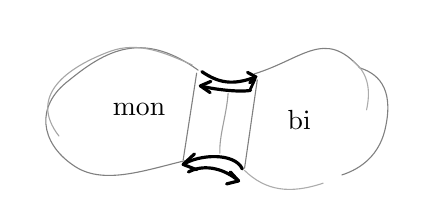
\begin{tikzpicture}[x=.0095cm,y=-.0095cm,line cap=round,line join=round]
  \draw[gray] (1075,177) .. controls (1000,123) and (951,151) .. (902,191) .. controls (857,225) and (864,274) .. (908,304) .. controls (946,331) and (1000,312) .. (1057,298);
  \draw[gray!70] (889,265) .. controls (848,212) and (898,174) .. (957,152) .. controls (995,138) and (1031,154) .. (1067,170);
  \draw[gray] (1150,182) .. controls (1215,162) and (1244,121) .. (1291,174) .. controls (1320,183) and (1337,207) .. (1324,259) .. controls (1316,289) and (1295,308) .. (1267,317);
  \draw[gray!65] (1242,328) .. controls (1197,343) and (1165,338) .. (1137,311);
  \draw[gray!65] (1282,165) .. controls (1304,182) and (1305,207) .. (1300,230);
  \draw[gray] (1073,181) -- (1055,297) (1154,190) -- (1137,308);
  \draw[gray!75] (1115,208) .. controls (1113,237) and (1103,264) .. (1104,288);
  \draw[line width=1.15pt] (1080,179) .. controls (1102,194) and (1121,198) .. (1152,186);
  \draw[line width=1.15pt] (1141,180) -- (1152,186) -- (1144,194);
  \draw[line width=1.0pt] (1151,189) -- (1144,204);
  \draw[line width=1.15pt] (1145,204) .. controls (1129,207) and (1092,202) .. (1078,198);
  \draw[line width=1.15pt] (1092,192) -- (1078,198) -- (1091,207);
  \draw[line width=1.15pt] (1134,309) .. controls (1124,287) and (1077,289) .. (1055,303);
  \draw[line width=1.15pt] (1070,289) -- (1055,303) -- (1073,310);
  \draw[line width=1.15pt] (1062,313) .. controls (1085,301) and (1112,310) .. (1129,325);
  \draw[line width=1.15pt] (1118,313) -- (1129,325) -- (1113,329);
  \node at (996,230) {mon}; \node at (1210,244) {bi};
\end{tikzpicture}}
Attachement de deux arêtes, l'une \unsure{monorive|monovive}, l'autre birive. On trouve \unsure{paire|pair} d'arêtes $\{a,a'\}$ \unsure{(}\deleted{\unsure{birives}}\inserted{monorives}) incidentes : une $=$ face \[\begin{aligned}f^{\ast}&=f'+f''-2\\ g&=g'\unsure{+|-}g''\end{aligned}\ \left|\begin{aligned}&\text{trois faces}\\ &\text{deviennent }1\end{aligned}\right.\]
\end{minipage}

\figure{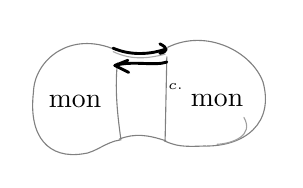
\begin{tikzpicture}[x=.011cm,y=-.011cm,line cap=round,line join=round]
  \draw[gray] (775,937) .. controls (722,914) and (681,949) .. (680,986) .. controls (674,1038) and (698,1063) .. (737,1057) .. controls (751,1056) and (764,1043) .. (780,1041);
  \draw[gray] (835,934) .. controls (880,912) and (932,939) .. (945,974) .. controls (958,1021) and (925,1049) .. (876,1048) .. controls (852,1049) and (845,1048) .. (831,1042);
  \draw[gray!75] (923,1015) .. controls (935,1036) and (910,1045) .. (892,1046);
  \draw[gray] (777,952) .. controls (773,987) and (779,1025) .. (781,1041) (834,945) -- (832,1042) (779,1040) .. controls (797,1033) and (812,1035) .. (833,1042);
  \draw[gray!65] (772,939) .. controls (795,950) and (815,946) .. (832,942);
  \draw[line width=1.05pt] (772,935) .. controls (788,942) and (810,944) .. (833,936);
  \draw[line width=1.05pt] (826,930) .. controls (836,935) and (835,939) .. (826,941);
  \draw[line width=1.05pt] (834,951) .. controls (820,956) and (794,949) .. (774,955);
  \draw[line width=1.05pt] (789,949) -- (774,955) -- (790,963);
  \node at (728,997) {mon}; \node at (892,995) {mon};
  \node[inner sep=0pt,font=\tiny] at (844,979) {$c$.};
\end{tikzpicture}}
Attachement de deux arêtes \deleted{\unsure{bifides|bifidées}}\unsure{monorives} on trouve \deleted{deux} paire d'arêtes monorives, incidentes à des faces distinctes

\[\begin{aligned}f&=f'+f''\\ \underline{g}&=g'+g''-1\end{aligned}\ \left|\begin{aligned}&\text{deux faces}\\ &\text{deviennent }2\end{aligned}\right.\]

\noindent\hfill\begin{minipage}{.55\linewidth}
\figure{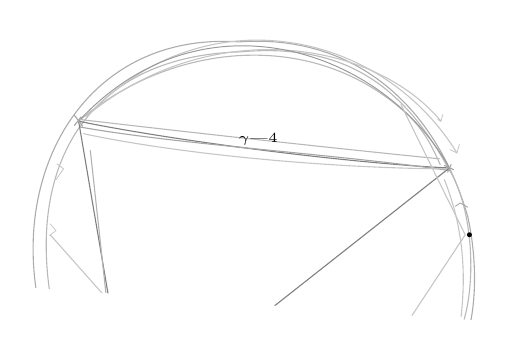
\begin{tikzpicture}[x=.0106cm,y=-.0106cm,line cap=round,line join=round]
  \clip (946,1308) -- (1489,1308) -- (1489,1659) -- (945,1619) -- cycle;
  \draw[gray!65] (958,1638) .. controls (925,1473) and (1019,1313) .. (1198,1325) .. controls (1335,1315) and (1433,1400) .. (1472,1534) .. controls (1483,1584) and (1482,1633) .. (1474,1667);
  \draw[gray!55] (975,1646) .. controls (940,1465) and (1024,1342) .. (1199,1337) .. controls (1321,1326) and (1392,1374) .. (1448,1475) .. controls (1478,1521) and (1483,1611) .. (1466,1663);
  \draw[gray!55] (1006,1420) .. controls (1114,1327) and (1287,1305) .. (1402,1414) .. controls (1422,1434) and (1431,1454) .. (1439,1472);
  \draw[gray!45] (1015,1414) .. controls (1166,1291) and (1360,1324) .. (1440,1420);
  \draw[gray!45] (1025,1405) .. controls (1165,1268) and (1371,1314) .. (1459,1458);
  \draw[gray!80,line width=.35pt] (1006,1420) .. controls (1156,1258) and (1373,1337) .. (1450,1476);
  \draw[gray] (1006,1420) .. controls (1122,1444) and (1338,1471) .. (1450,1476);
  \draw[gray!70] (1008,1427) .. controls (1126,1448) and (1310,1459) .. (1450,1479);
  \draw[gray!55] (1008,1418) .. controls (1153,1435) and (1327,1454) .. (1438,1465);
  \draw[gray!45] (1012,1435) .. controls (1139,1462) and (1327,1477) .. (1450,1477);
  \draw[gray] (1006,1420) -- (1043,1637) (1450,1476) -- (1237,1644);
  \draw[gray!60] (1020,1455) -- (1040,1638);
  \draw[gray!45] (972,1556) -- (1043,1636) (1392,1400) -- (1469,1556) -- (1405,1653);
  \draw[gray!45] (1444,1490) .. controls (1464,1540) and (1471,1593) .. (1464,1654);
  \draw[gray!70,line width=.4pt] (1001,1413) -- (1011,1426) (1001,1425) -- (1009,1415) (1444,1473) -- (1455,1478) (1448,1481) -- (1452,1472);
  \draw[gray!70,line width=.3pt] (1457,1522) -- (1463,1518) -- (1472,1523);
  \draw[gray!45,line width=.3pt] (1436,1418) -- (1440,1420) -- (1442,1412);
  \draw[gray!45,line width=.3pt] (1451,1454) -- (1459,1458) -- (1462,1448);
  \draw[gray!45,line width=.3pt] (980,1471) -- (988,1477) -- (979,1490);
  \draw[gray!40,line width=.3pt] (972,1543) -- (979,1551) -- (971,1557);
  \fill (1474,1556) circle (3);
  \node[inner sep=0pt,font=\tiny] at (1221,1442) {\unsure{$\gamma$|$4$}};
\end{tikzpicture}}
\end{minipage}
% archive sheet number: 53

\scanpage{55}
\figure{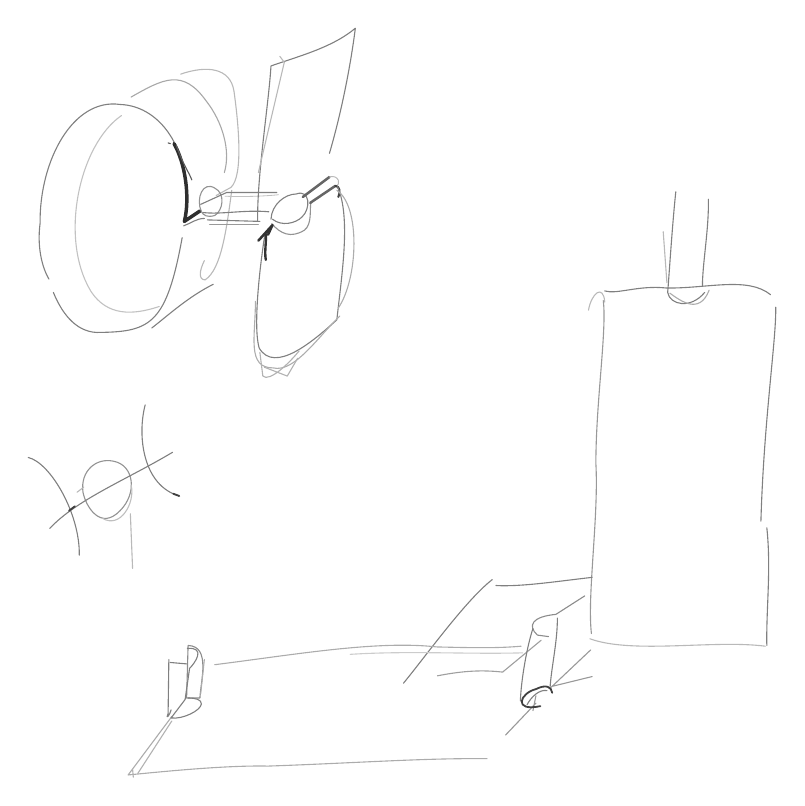
\begin{tikzpicture}[x=.0094cm,y=-.0094cm,line cap=round,line join=round]
  \draw[gray] (398,480) .. controls (410,393) and (368,327) .. (310,325) .. controls (247,316) and (201,400) .. (202,486) .. controls (198,516) and (204,544) .. (214,561);
  \draw[gray] (220,579) .. controls (233,611) and (254,635) .. (284,633) .. controls (352,632) and (373,620) .. (394,505);
  \draw[gray!48] (312,340) .. controls (255,379) and (227,506) .. (271,578) .. controls (293,611) and (327,610) .. (363,598);
  \draw[gray!68] (325,315) .. controls (369,290) and (395,276) .. (427,321) .. controls (448,348) and (460,387) .. (451,417);
  \draw[gray!55] (392,284) .. controls (427,272) and (459,275) .. (464,307) .. controls (470,350) and (477,421) .. (460,437) -- (440,448);
  \draw[gray!55] (461,441) .. controls (454,493) and (447,548) .. (425,562) .. controls (416,562) and (417,550) .. (424,536);
  \draw[gray] (436,568) .. controls (402,585) and (375,610) .. (353,627);
  \draw[black!82,line width=1.25pt] (383,378) .. controls (398,404) and (405,450) .. (397,483) -- (418,469);
  \draw[black!64] (375,377) -- (378,378) (386,380) .. controls (395,406) and (404,418) .. (407,427);
  \draw[gray] (396,489) .. controls (405,486) and (413,479) .. (424,479);
  \draw[gray!85] (420,470) .. controls (412,452) and (422,428) .. (438,438) .. controls (453,445) and (449,469) .. (438,475) .. controls (428,478) and (423,475) .. (420,470);
  \draw[gray] (419,460) -- (454,444) -- (522,444) (422,471) .. controls (447,474) and (478,467) .. (511,470) (428,481) -- (499,483);
  \draw[gray!48,line width=.3pt] (452,449) .. controls (478,450) and (504,449) .. (524,447);
  \draw[gray!80] (431,487) -- (497,487);
  \draw[gray] (514,480) .. controls (515,460) and (533,446) .. (548,446) .. controls (567,439) and (568,466) .. (556,477) .. controls (547,486) and (528,490) .. (516,480);
  \draw[gray!85] (515,486) .. controls (527,500) and (541,506) .. (559,495) .. controls (570,487) and (566,466) .. (568,457);
  \draw[black!60,line width=.9pt] (557,450) -- (593,423) (567,458) -- (601,435);
  \draw[gray!55,line width=.35pt] (593,423) .. controls (605,419) and (610,434) .. (601,435);
  \draw[black!75,line width=.75pt] (601,435) .. controls (607,435) and (608,444) .. (605,450);
  \draw[gray] (496,483) .. controls (495,421) and (511,324) .. (514,273) .. controls (547,261) and (596,249) .. (628,222) .. controls (621,277) and (608,340) .. (593,391);
  \draw[gray!55] (497,417) -- (532,268) -- (526,260);
  \draw[gray] (506,499) .. controls (498,550) and (490,626) .. (498,654) .. controls (519,690) and (572,644) .. (603,616) .. controls (610,552) and (622,478) .. (604,436);
  \draw[gray!64] (603,441) .. controls (635,462) and (632,560) .. (605,600) (493,591) .. controls (493,639) and (481,681) .. (517,681) .. controls (546,688) and (579,637) .. (607,611);
  \draw[gray!60] (499,660) -- (503,692) .. controls (512,701) and (540,673) .. (552,658) (505,680) -- (536,692) -- (550,668);
  \draw[black!80,line width=.9pt] (497,509) -- (516,488) -- (510,501);
  \draw[black!80,line width=.85pt] (507,500) .. controls (508,510) and (505,523) .. (507,535);
  \draw[gray] (186,802) .. controls (216,809) and (256,878) .. (255,934);
  \draw[gray] (344,731) .. controls (333,773) and (341,840) .. (390,854);
  \draw[gray!85] (260,849) .. controls (256,820) and (278,802) .. (301,807) .. controls (329,812) and (334,850) .. (310,874) .. controls (284,901) and (264,869) .. (260,849);
  \draw[gray!50] (286,884) .. controls (310,899) and (331,864) .. (325,839);
  \draw[gray] (215,898) .. controls (251,859) and (319,832) .. (381,795);
  \draw[gray!55] (252,849) -- (261,842) (324,878) -- (327,952);
  \draw[black!75,line width=.65pt] (241,874) -- (249,868);
  \draw[black!75,line width=.65pt] (382,851) -- (390,854);
  \draw[gray] (965,577) .. controls (982,582) and (1010,569) .. (1048,573) .. controls (1103,574) and (1158,557) .. (1189,582);
  \draw[gray] (1196,599) .. controls (1197,642) and (1180,750) .. (1176,888) (1184,897) .. controls (1190,953) and (1183,1007) .. (1184,1056);
  \draw[gray!80] (963,590) .. controls (968,630) and (953,727) .. (953,810) .. controls (957,881) and (941,990) .. (947,1040);
  \draw[gray!55] (945,1047) .. controls (1003,1068) and (1112,1048) .. (1182,1057);
  \draw[gray!55] (943,603) .. controls (947,580) and (963,567) .. (965,592) (1044,497) -- (1049,566);
  \draw[gray] (1061,443) .. controls (1056,490) and (1052,556) .. (1050,579) .. controls (1053,596) and (1081,602) .. (1100,579);
  \draw[gray] (1105,453) .. controls (1106,492) and (1097,540) .. (1097,570);
  \draw[gray!65] (1053,580) .. controls (1067,590) and (1093,610) .. (1106,576);
  \draw[gray] (693,1107) .. controls (722,1072) and (777,995) .. (813,967) (818,975) .. controls (852,977) and (903,969) .. (948,964);
  \draw[gray!75] (739,1097) .. controls (775,1090) and (800,1089) .. (827,1092) -- (879,1049);
  \draw[gray!65] (438,1082) .. controls (549,1068) and (657,1049) .. (738,1058) .. controls (782,1059) and (819,1060) .. (852,1057);
  \draw[gray!40] (621,1068) .. controls (701,1063) and (776,1068) .. (854,1066);
  \draw[gray!65] (380,1152) -- (321,1231) .. controls (391,1224) and (460,1218) .. (510,1219) .. controls (626,1215) and (722,1208) .. (806,1209);
  \draw[gray!60] (327,1223) -- (328,1234) (334,1229) -- (380,1158);
  \draw[gray] (376,1075) -- (375,1148) .. controls (371,1158) and (378,1149) .. (379,1143) (378,1079) -- (401,1081);
  \draw[gray!90] (402,1056) .. controls (433,1057) and (419,1104) .. (418,1127) -- (400,1127) -- (402,1056);
  \draw[gray] (401,1060) .. controls (427,1058) and (411,1080) .. (404,1087) -- (398,1129) -- (379,1154) .. controls (395,1156) and (419,1144) .. (420,1135) .. controls (420,1129) and (412,1127) .. (402,1127);
  \draw[gray!65] (424,1075) -- (419,1121);
  \draw[gray!90] (938,989) -- (899,1014) .. controls (867,1017) and (860,1029) .. (874,1042) -- (889,1044);
  \draw[gray] (901,1019) .. controls (901,1052) and (893,1084) .. (891,1114) (868,1033) .. controls (860,1057) and (852,1102) .. (851,1131);
  \draw[gray!80] (831,1177) -- (872,1134) (868,1144) -- (872,1124) (891,1114) -- (946,1062) (895,1111) -- (948,1098);
  \draw[black!75,line width=.65pt] (878,1138) .. controls (840,1146) and (851,1120) .. (872,1115) .. controls (886,1108) and (893,1112) .. (894,1120);
  \draw[gray] (860,1136) .. controls (866,1125) and (877,1115) .. (887,1117);
\end{tikzpicture}}
% archive sheet number: 54
